\documentclass[UTF8]{ctexart}[a4paper,10pt]
\usepackage[thmmarks]{ntheorem}
\usepackage{amsmath}
\usepackage{amsfonts,amssymb} 
\usepackage{thmtools}
\usepackage[hmargin=2.5cm,vmargin=2.5cm]{geometry}
\usepackage{tikz-cd,tikz}
\usepackage{graphicx,float}
\usepackage{fancyhdr}
\usepackage{fourier-orns}
\usepackage{quiver}

%声明环境
\newtheorem{example}{例}[section]              
\newtheorem{algorithm}{算法}[subsection]
\newtheorem{theorem}{定理}[section]            
\newtheorem{definition}{定义}[section]
\newtheorem{axiom}{公理}[section]
\newtheorem{property}{性质}[section]
\newtheorem{proposition}{命题}[section]
\newtheorem{lemma}[theorem]{引理}
\newtheorem{corollary}[theorem]{推论}
{
    \theoremheaderfont{\sffamily}
    \newtheorem*{remark}{注解} 
}
\newtheorem{condition}{条件}
\newtheorem{conclusion}{结论}[section]
\newtheorem{assumption}{假设}
{
\theoremstyle{nonumberplain}
\theoremheaderfont{\bfseries}
\theorembodyfont{\normalfont}
\theoremsymbol{\mbox{$\Box$}}
\newtheorem{proof}{证明}
}
%定义命令
\def\N{\mathbb{N}}
\def\Z{\mathbb{Z}}
\def\Q{\mathbb{Q}}
\def\R{\mathbb{R}}
\def\C{\mathbb{C}}
\def\S{\mathbb{S}}
\def\D{\mathbb{D}}
\def\H{\mathbb{H}}
%外测度
\def\outmQ{m_*(Q)}

%页眉设计
\renewcommand 
\headrule{
\hrulefill
\raisebox{-2.1pt}
{\quad{\FourierOrns M T S N}\quad}
\hrulefill}
\pagestyle{fancy}

%超链接红色
\usepackage[colorlinks,linkcolor=red]{hyperref}

\usepackage{enumerate}


\title{\textbf{Algebra:Chapter 0}:Set and Categories}
\author{颜成子游}
\begin{document}
\maketitle
\tableofcontents
\newpage
Algebra:Chapter 0 是一本非常详细的代数学教材,其详实程度
远远大于通常的代数学教材。我们将从集合论和范畴论开始,一点一点
地搭建起初等的代数体系,从而为之后的代数学习打下基础。

在这一份pdf中,我们将聚焦于本书的第一章:集
合论与范畴论(初等的)。
\section{朴素集合论}
\subsection{一些记号和概念}
朴素集合论本质上是一种术语和记号,它将帮助我们表达
许多概念,定理,证明。尽管存在罗素悖论,但在这本书中我们并不会遇到
这样的情况,从而我们将不去讲“ZF"系统。

作为一名数学系本科生,以下的概念应当是不陌生的:
\begin{definition}
    我们不加定义的给出下面若干概念:
    \begin{enumerate}
        \item 集合、元素
        \item 集合拥有的性质:明确性,无序性,不重复性
        \item 表述集合的方法:
        $$
        P=\{p \in S|p \quad \text{satisfies property} \quad P\}
        $$
        \item 多集合(允许元素重复的集合)
        \item 单点集
        \item 集合与集合之间的关系:包含与子集,真子集,空集,幂集($\mathcal{P}(S)$)
    \end{enumerate}
\end{definition}


\begin{definition}[集合之间的运算]
    下面这些概念也是为人熟知的:
    \begin{enumerate}
        \item 并
        \item 交
        \item 差
        \item 不交并
        \item 笛卡尔积
        \item 由等价关系产生的商
    \end{enumerate}
\end{definition}
\subsection{集合之间的函数}
对于一名知道一点高中数学的人来讲,函数的概念也应当是刻在DNA之中的。
然而“函数”总给我们一种动态的感觉。事实上,这是没有必要的:
\begin{definition}
    一个从$A$到$B$的函数$f$是笛卡尔直积$A \times B$的子集:
    $$
    \Gamma_f=\{(a,b)\in A\times B|b=f(a)\}
    $$
    从定义看出,若有
    $$
    (a,b) (a,b^*)
    $$
    同属于一个$\Gamma_f$,那一定有$b=b^*$。另外
    $$
    \{a|(a,b)\in \Gamma_f\}=A
    $$
   我们把$\Gamma_f$称为$f$的图像。
\end{definition}
我们也有符号:
\begin{figure}[H]
    \centering
    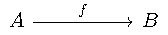
\includegraphics[scale=1.2]{functionpre.pdf}
\end{figure}
这样的符号将在之后经常使用。


\begin{definition}
    接下来的几个概念和记号也是不陌生的:
    \begin{enumerate}
        \item 恒等映射,映入映射,限制映射
        \item 将$A$到$B$的所有映射构成的集合记为:
        $$
        B^A
        $$
        \item 指标集(从数列抽象而来)
    \end{enumerate}
\end{definition}

接下来我们将讨论一些新的东西。尽管集合间的函数是足够简单的,
但是我们也得到一些非常好的东西。

值得注意的是,我们将使用所谓“交换图”来表示我们的结果。

\begin{definition}[函数的复合]
    如果$f:A \to B$和$g:B \to C$是函数,那么函数复合
    $g \circ f$是满足下列交换图成立的映射:
    \begin{figure}[h]
        \centering
        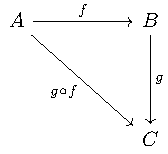
\includegraphics[scale=0.8]{composition.pdf}
    \end{figure} 
\end{definition}
\begin{theorem}
    函数的复合是交换的。即若有$f:A \to B$,
    $g:B \to C$,$h:C \to D$,下面的交换图是成立的:
    \begin{figure}[H]
        \centering
        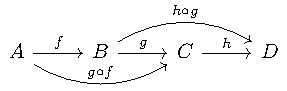
\includegraphics[scale=1.2]
        {associative.pdf}

    \end{figure}
\end{theorem}

恒等映射与任何函数复合都不会改变原来的函数。

\begin{definition}[单射,满射,双射(一)]
    \quad

    单射:$f(a)=f(a^*) \Rightarrow a=a^*$

    满射:$\forall b \in B, \exists a \in A:f(a)=b$

    双射:既是单射又是满射.

    单射记为:$\hookrightarrow$,满射记为$\twoheadrightarrow $
\end{definition}
\begin{definition}[单射,满射,双射(二)]
    \quad
    
    称$g$是$f$的左逆,如果图:
    \begin{figure}[h]
        \centering
        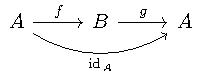
\includegraphics[scale=1.2]
        {leftinverse.pdf}
    \end{figure}

    成立

    称$g$是$f$的右逆,如果图:
    \begin{figure}[h]
        \centering
        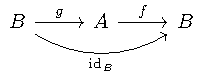
\includegraphics[scale=1.2]
        {rightinverse.pdf}
    \end{figure}

    成立


    单射:有左逆。

    满射:有右逆。

    双射:既有左逆又有右逆。
\end{definition}
我们将不去验证两种定义的等价性。但值得注意的是,定义二是更本质的东西,
因为它不去设计$A$,$B$具体有什么元素。如果我们考虑的东西不是集合(范畴论)
,那么定义二将成为唯一的定义方式。

需要指出,如果只是单射、满射,那么其左逆(右逆)一般是不唯一的。但是
如果是双射,那么其左逆和右逆不仅唯一,而且相等:
$$
g\circ f=\text{id}_A
$$
$$
f\circ h =\text{id}_B
$$

则:$$
g=g \circ \text{id}_B    = g \circ f \circ h =\text{id}_A \circ h=h
$$
\begin{definition}[单态射与满态射]
    \quad

    一个映射$f:A \to B$是一个单态射,如果对于所有的集合$Z$和所有
    函数$\alpha,\alpha^*: Z \to A$,都有:
    $$
    f \circ \alpha=f \circ \alpha^* \Rightarrow \alpha=\alpha^*
    $$

    一个映射$f:A \to B$是一个满态射,如果对于所有的集合$M$和所有的函数
    $\beta,\beta^*: B \to M$,都有:
    $$
    \beta \circ f=\beta^* \circ f \Rightarrow \beta =\beta^*
    $$
\end{definition}
我们不加证明的指出以下结论。请注意,只有在集合的意义下,下面的结论
才是显然成立的(不能任何时候都认为他们一样)
\begin{proposition}
    一个映射是单射当且仅当其是单态射;一个映射是满射当且仅当其是满态射。
\end{proposition}
接下里给出一个小例子。
\begin{example}
    如果$A,B$是集合,那么存在自然映射$\pi_A,\pi_B$:
    \begin{figure}[h]
        \centering
        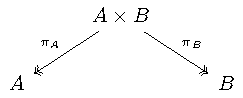
\includegraphics{naturalprojection.pdf}
    \end{figure}

    其中,$\pi_A((a,b))=a,\pi_B((a,b))=b$。显然都是满射。
\end{example}
现在给出一个极其有价值的定理:
\begin{theorem}
    设$f:A \to B $是一个映射,那么$f$可以按照如下交换图分解:
    \begin{figure}[h]
        \centering
        \begin{tikzcd}
            A & {(A/\sim)} & {\text{im}f} & B
            \arrow[two heads, from=1-1, to=1-2]
            \arrow[hook, from=1-3, to=1-4]
            \arrow["f", curve={height=-18pt}, from=1-1, to=1-4]
            \arrow["{\tilde{f}}", from=1-2, to=1-3]
            \arrow["\sim"', from=1-2, to=1-3]
        \end{tikzcd}
    \end{figure}
    
    其中$\sim$是等价关系:$f(a)=f(b) \Leftrightarrow a \sim b$

    另外$\tilde{f}([a]_{\sim}):=f(a)$

    其余的两个映射,一个是自然映射$A \to A/\sim$,一个是内射$\text{im}f \to B$.

\end{theorem}
\begin{proof}
    显然。
\end{proof}
\section{范畴论}
范畴论是一种语言,其关注于所谓的“结构”,而非“意义”。这一点在之后的
学习中会逐渐凸显。集合是一种范畴,但范畴能描述更多更有意思的东西。
同时,在范畴中我们也能意识到哪些性质是“基本”的,哪些性质是特殊的代数对象特有的。
\begin{definition}
    一个范畴$\mathsf{C}$包含:
    \begin{enumerate}[*]
        \item 一个由对象所组成的类$\text{Obj}(\mathsf{C})$
        \item 对于任何两个对象$A,B$,存在一个集合$\text{Hom}_{\mathsf{C}}(A,B)$
        ,称为$A,B$之间的态射,并且拥有以下性质:
        \begin{enumerate}[$\bullet$]
            \item 对于每个对象$A$,态射集合$Hom(A,A)$非空,包含一个元素$1_A$,称为
            $A$的恒等态射。
            \item 
        \end{enumerate}
    \end{enumerate}
\end{definition}
\end{document}